\begin{frame}
\frametitle{Planificación del proyecto}
\framesubtitle{Sampling System GUI (SSG)}
\begin{itemize}
    \item Proyecto perteneciente al ALMA-UTFSM Group.
	\item Se considerarán algunos aspectos del proyecto.
	\item Se utilizarán las mismas herramientas con las cuales fue desarrollado.
\end{itemize}
\begin{center}
	
\includegraphics[width=0.2\textwidth]{img/alma}
\end{center}
\end{frame}

\begin{frame}
\frametitle{Planificación del proyecto}
\framesubtitle{Sampling System GUI (SSG)}
\begin{itemize}
    \item Contexto:
	\begin{itemize}
		\item Antenas del proyecto ALMA formadas por componentes.
		\item Los componentes están formados por propiedades.
		\item Cada propiedades va obteniendo valores.
		\item SSG obtiene esos valores y los dibuja. (comportamiento)
	\end{itemize}
\end{itemize}
\begin{center}
	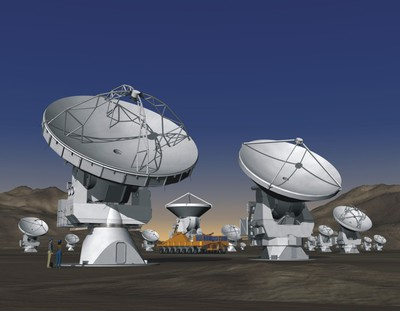
\includegraphics[width=0.2\textwidth]{img/antena}
\end{center}
\end{frame}

